%%%%%%%%%%%%%%%%%%%%%%%%%%%%%%%%%%%%%%%%%%%%%%%%%%%%%%%%%%%%%%%%%%%%%%%%%%%%%%%%%%%%%%%%%%%%%%%%
%
% CS484 Written Question Template
%
% Acknowledgements:
% The original code is written by Prof. James Tompkin (james_tompkin@brown.edu).
% The second version is revised by Prof. Min H. Kim (minhkim@kaist.ac.kr).
%
% This is a LaTeX document. LaTeX is a markup language for producing
% documents. Your task is to fill out this document, then to compile
% it into a PDF document.
%
%
% TO COMPILE:
% > pdflatex thisfile.tex
%
% If you do not have LaTeX and need a LaTeX distribution:
% - Personal laptops (all common OS): www.latex-project.org/get/
% - We recommend latex compiler miktex (https://miktex.org/) for windows,
%   macTex (http://www.tug.org/mactex/) for macOS users.
%   And TeXstudio(http://www.texstudio.org/) for latex editor.
%   You should install both compiler and editor for editing latex.
%   The another option is Overleaf (https://www.overleaf.com/) which is
%   an online latex editor.
%
% If you need help with LaTeX, please come to office hours.
% Or, there is plenty of help online:
% https://en.wikibooks.org/wiki/LaTeX
%
% Good luck!
% Min and the CS484 staff
%
%%%%%%%%%%%%%%%%%%%%%%%%%%%%%%%%%%%%%%%%%%%%%%%%%%%%%%%%%%%%%%%%%%%%%%%%%%%%%%%%%%%%%%%%%%%%%%%%
%
% How to include two graphics on the same line:
%
% \includegraphics[width=0.49\linewidth]{yourgraphic1.png}
% \includegraphics[width=0.49\linewidth]{yourgraphic2.png}
%
% How to include equations:
%
% \begin{equation}
% y = mx+c
% \end{equation}
%
%%%%%%%%%%%%%%%%%%%%%%%%%%%%%%%%%%%%%%%%%%%%%%%%%%%%%%%%%%%%%%%%%%%%%%%%%%%%%%%%%%%%%%%%%%%%%%%%

\documentclass[11pt]{article}

\usepackage[english]{babel}
\usepackage[utf8]{inputenc}
\usepackage[colorlinks = true,
            linkcolor = blue,
            urlcolor  = blue]{hyperref}
\usepackage[a4paper,margin=1.5in]{geometry}
\usepackage{stackengine,graphicx}
\usepackage{fancyhdr}
\setlength{\headheight}{15pt}
\usepackage{microtype}
\usepackage{times}

% From https://ctan.org/pkg/matlab-prettifier
\usepackage[numbered,framed]{matlab-prettifier}

\frenchspacing
\setlength{\parindent}{0cm} % Default is 15pt.
\setlength{\parskip}{0.3cm plus1mm minus1mm}

\pagestyle{fancy}
\fancyhf{}
\lhead{Homework 4 Questions}
\rhead{CS 484}
\rfoot{\thepage}

\date{}

\title{\vspace{-1cm}Homework 4 Questions}


\begin{document}
\maketitle
\vspace{-3cm}
\thispagestyle{fancy}

\section*{Instructions}
\begin{itemize}
  \item 4 questions.
  \item Write code where appropriate.
  \item Feel free to include images or equations.
  \item Please make this document anonymous.
  \item \textbf{Please use only the space provided and keep the page breaks.} Please do not make new pages, nor remove pages. The document is a template to help grading.
  \item If you really need extra space, please use new pages at the end of the document and refer us to it in your answers.
\end{itemize}

\section*{Questions}

\paragraph{Q1:} Imagine we were tasked with designing a feature point which could match all of the following three pairs of images. Which real world phenomena and camera effects might cause us problems?
Use the MATLAB function \href{https://www.mathworks.com/help/images/ref/corner.html}{$corner$} to investigate. $corner(I,1000)$.

\emph{RISHLibrary} | \emph{Chase} | \emph{LaddObservatory}

%%%%%%%%%%%%%%%%%%%%%%%%%%%%%%%%%%%
\paragraph{A1:}

The \emph{RISHLibrary} image pair poses two problems. The first is the difference in illuminance/color tone. Algorithms like SIFT might help achieve illuminance invariance, but the difference color tone might be the cause of problems.

One of the images in the \emph{Chase} pair is blurred presumably due to camera motion. This could distract the algorithm because the blur might appear as different features.

Finally, the \emph{LaddObservatory} image pairs are different in scale, as one image seems to be a zoomed version of a portion of the other. To detect and match two points in the images, the feature would have to be invariant to scale.

\pagebreak
\paragraph{A1:} This page includes corner detection outputs for the given image pairs

\begin{figure}[h]
    \centering
    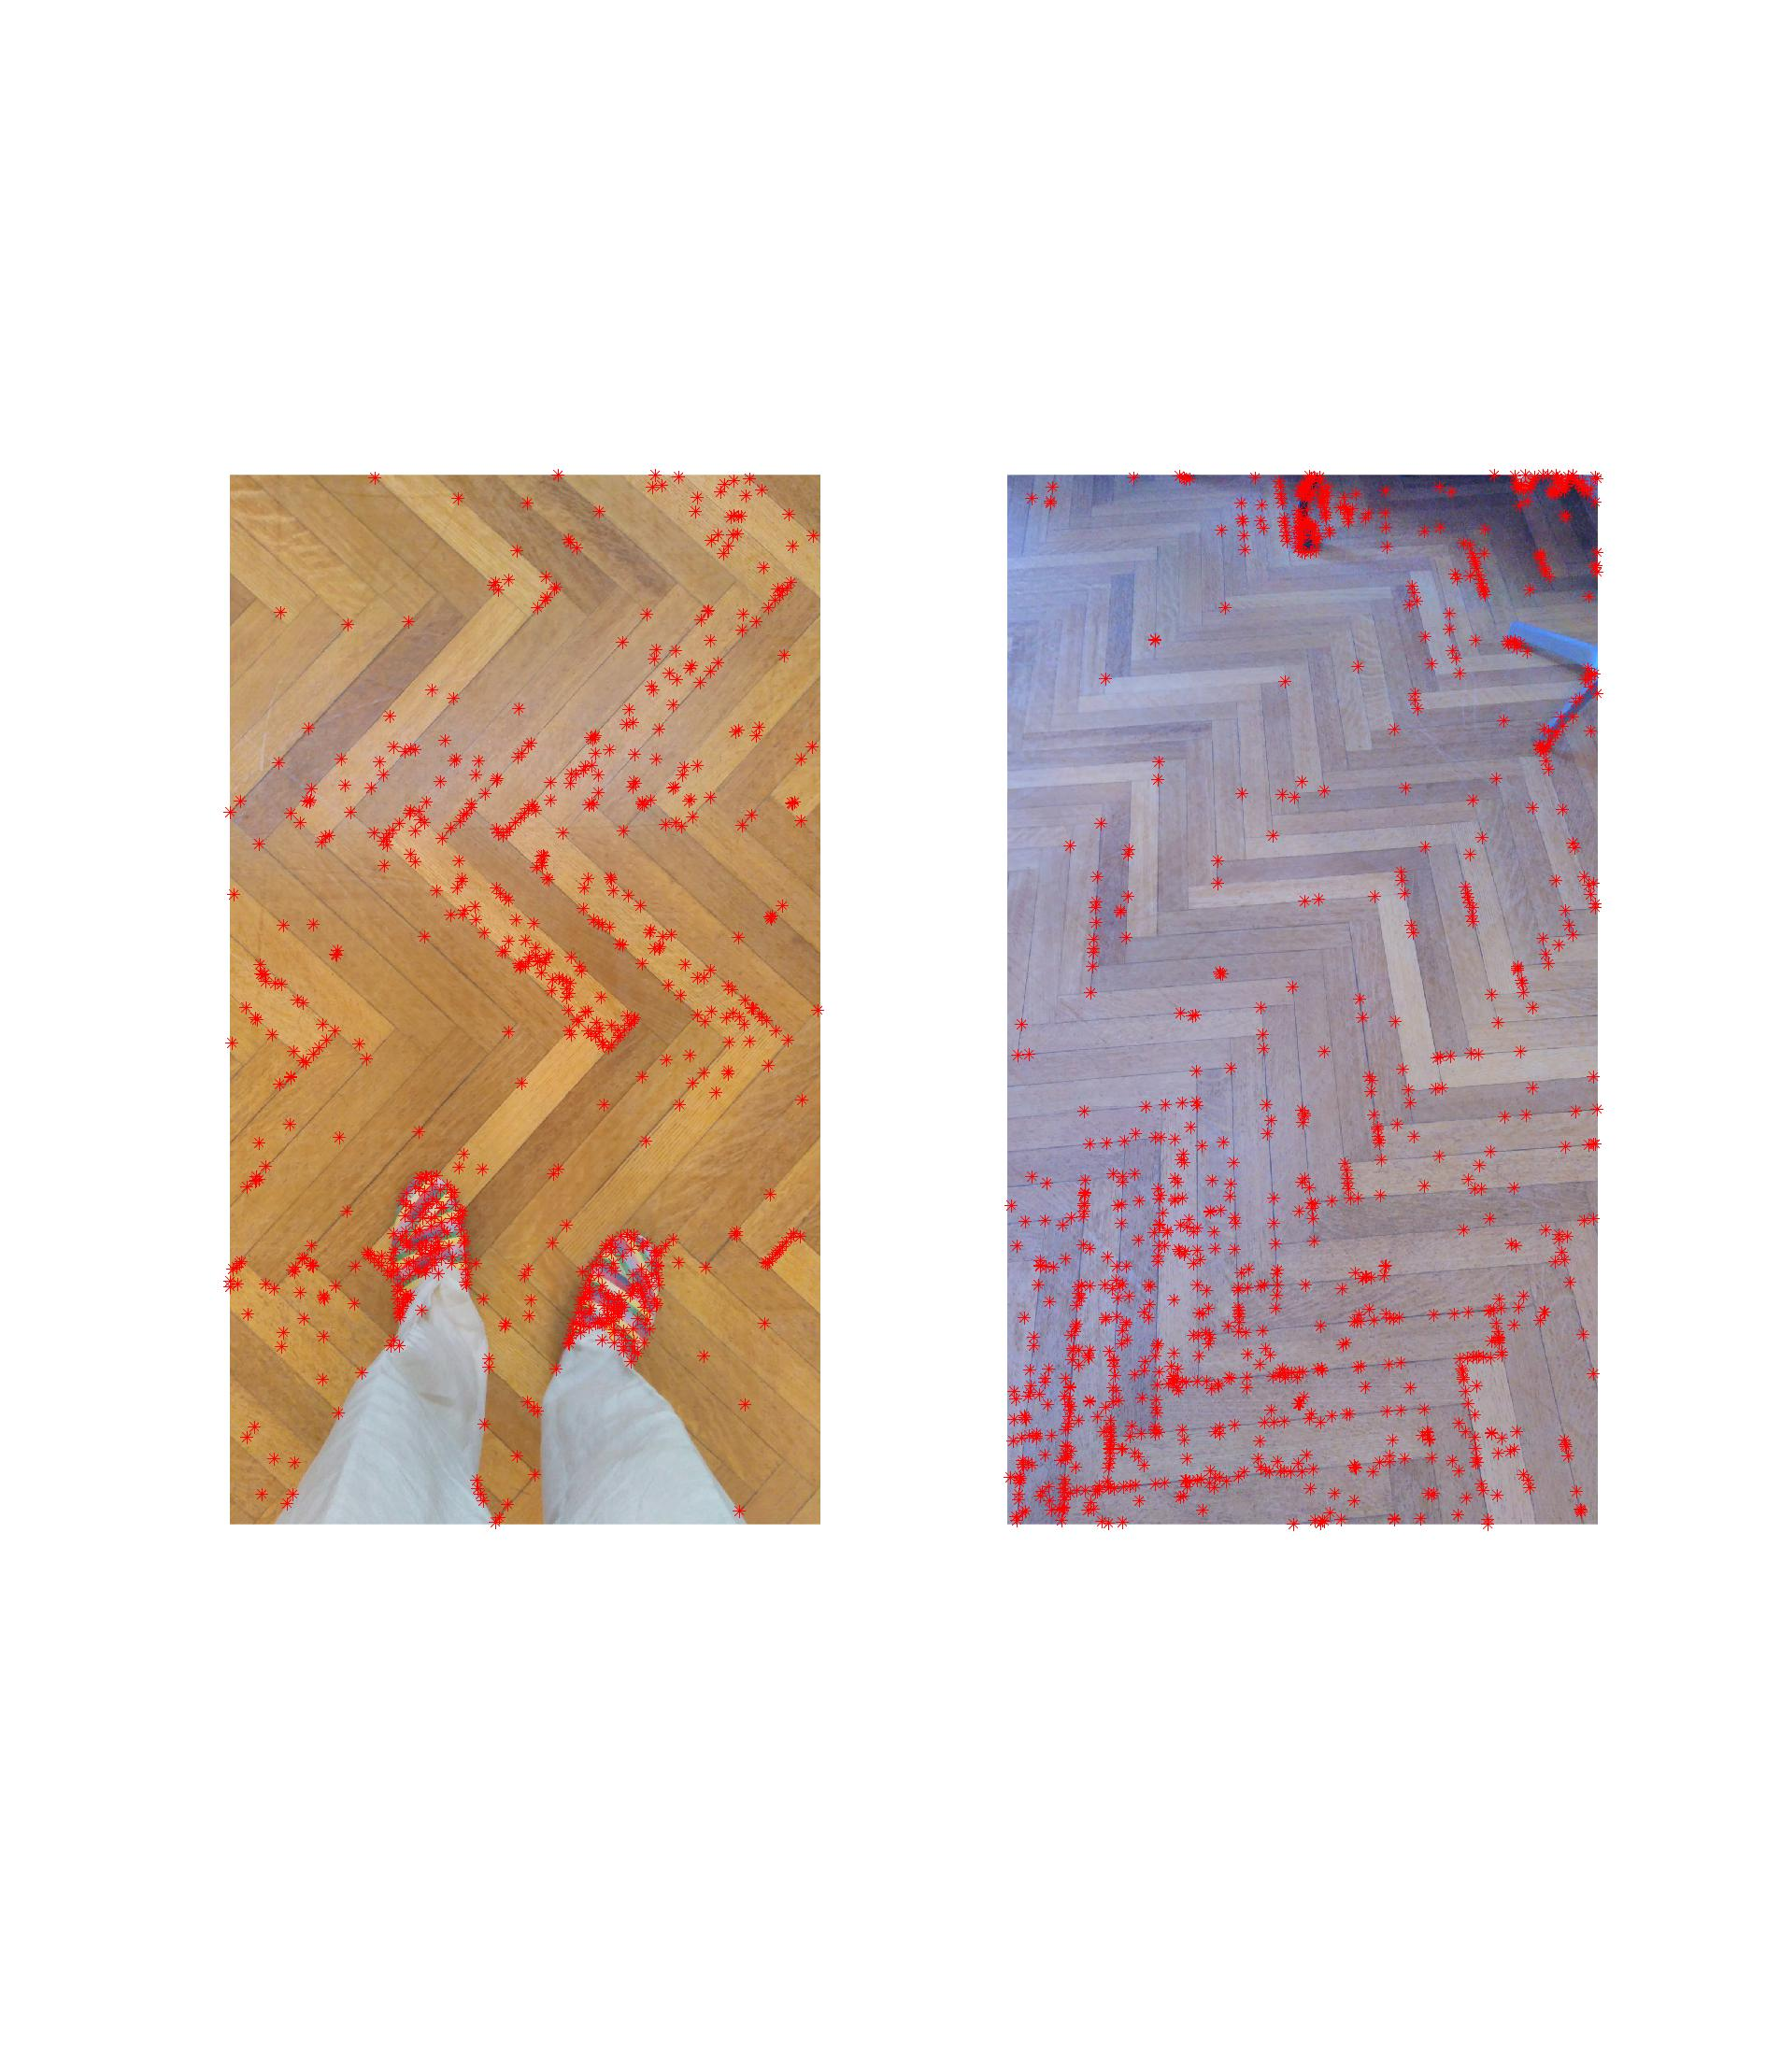
\includegraphics[width=5cm]{outputs/Library.jpg}
    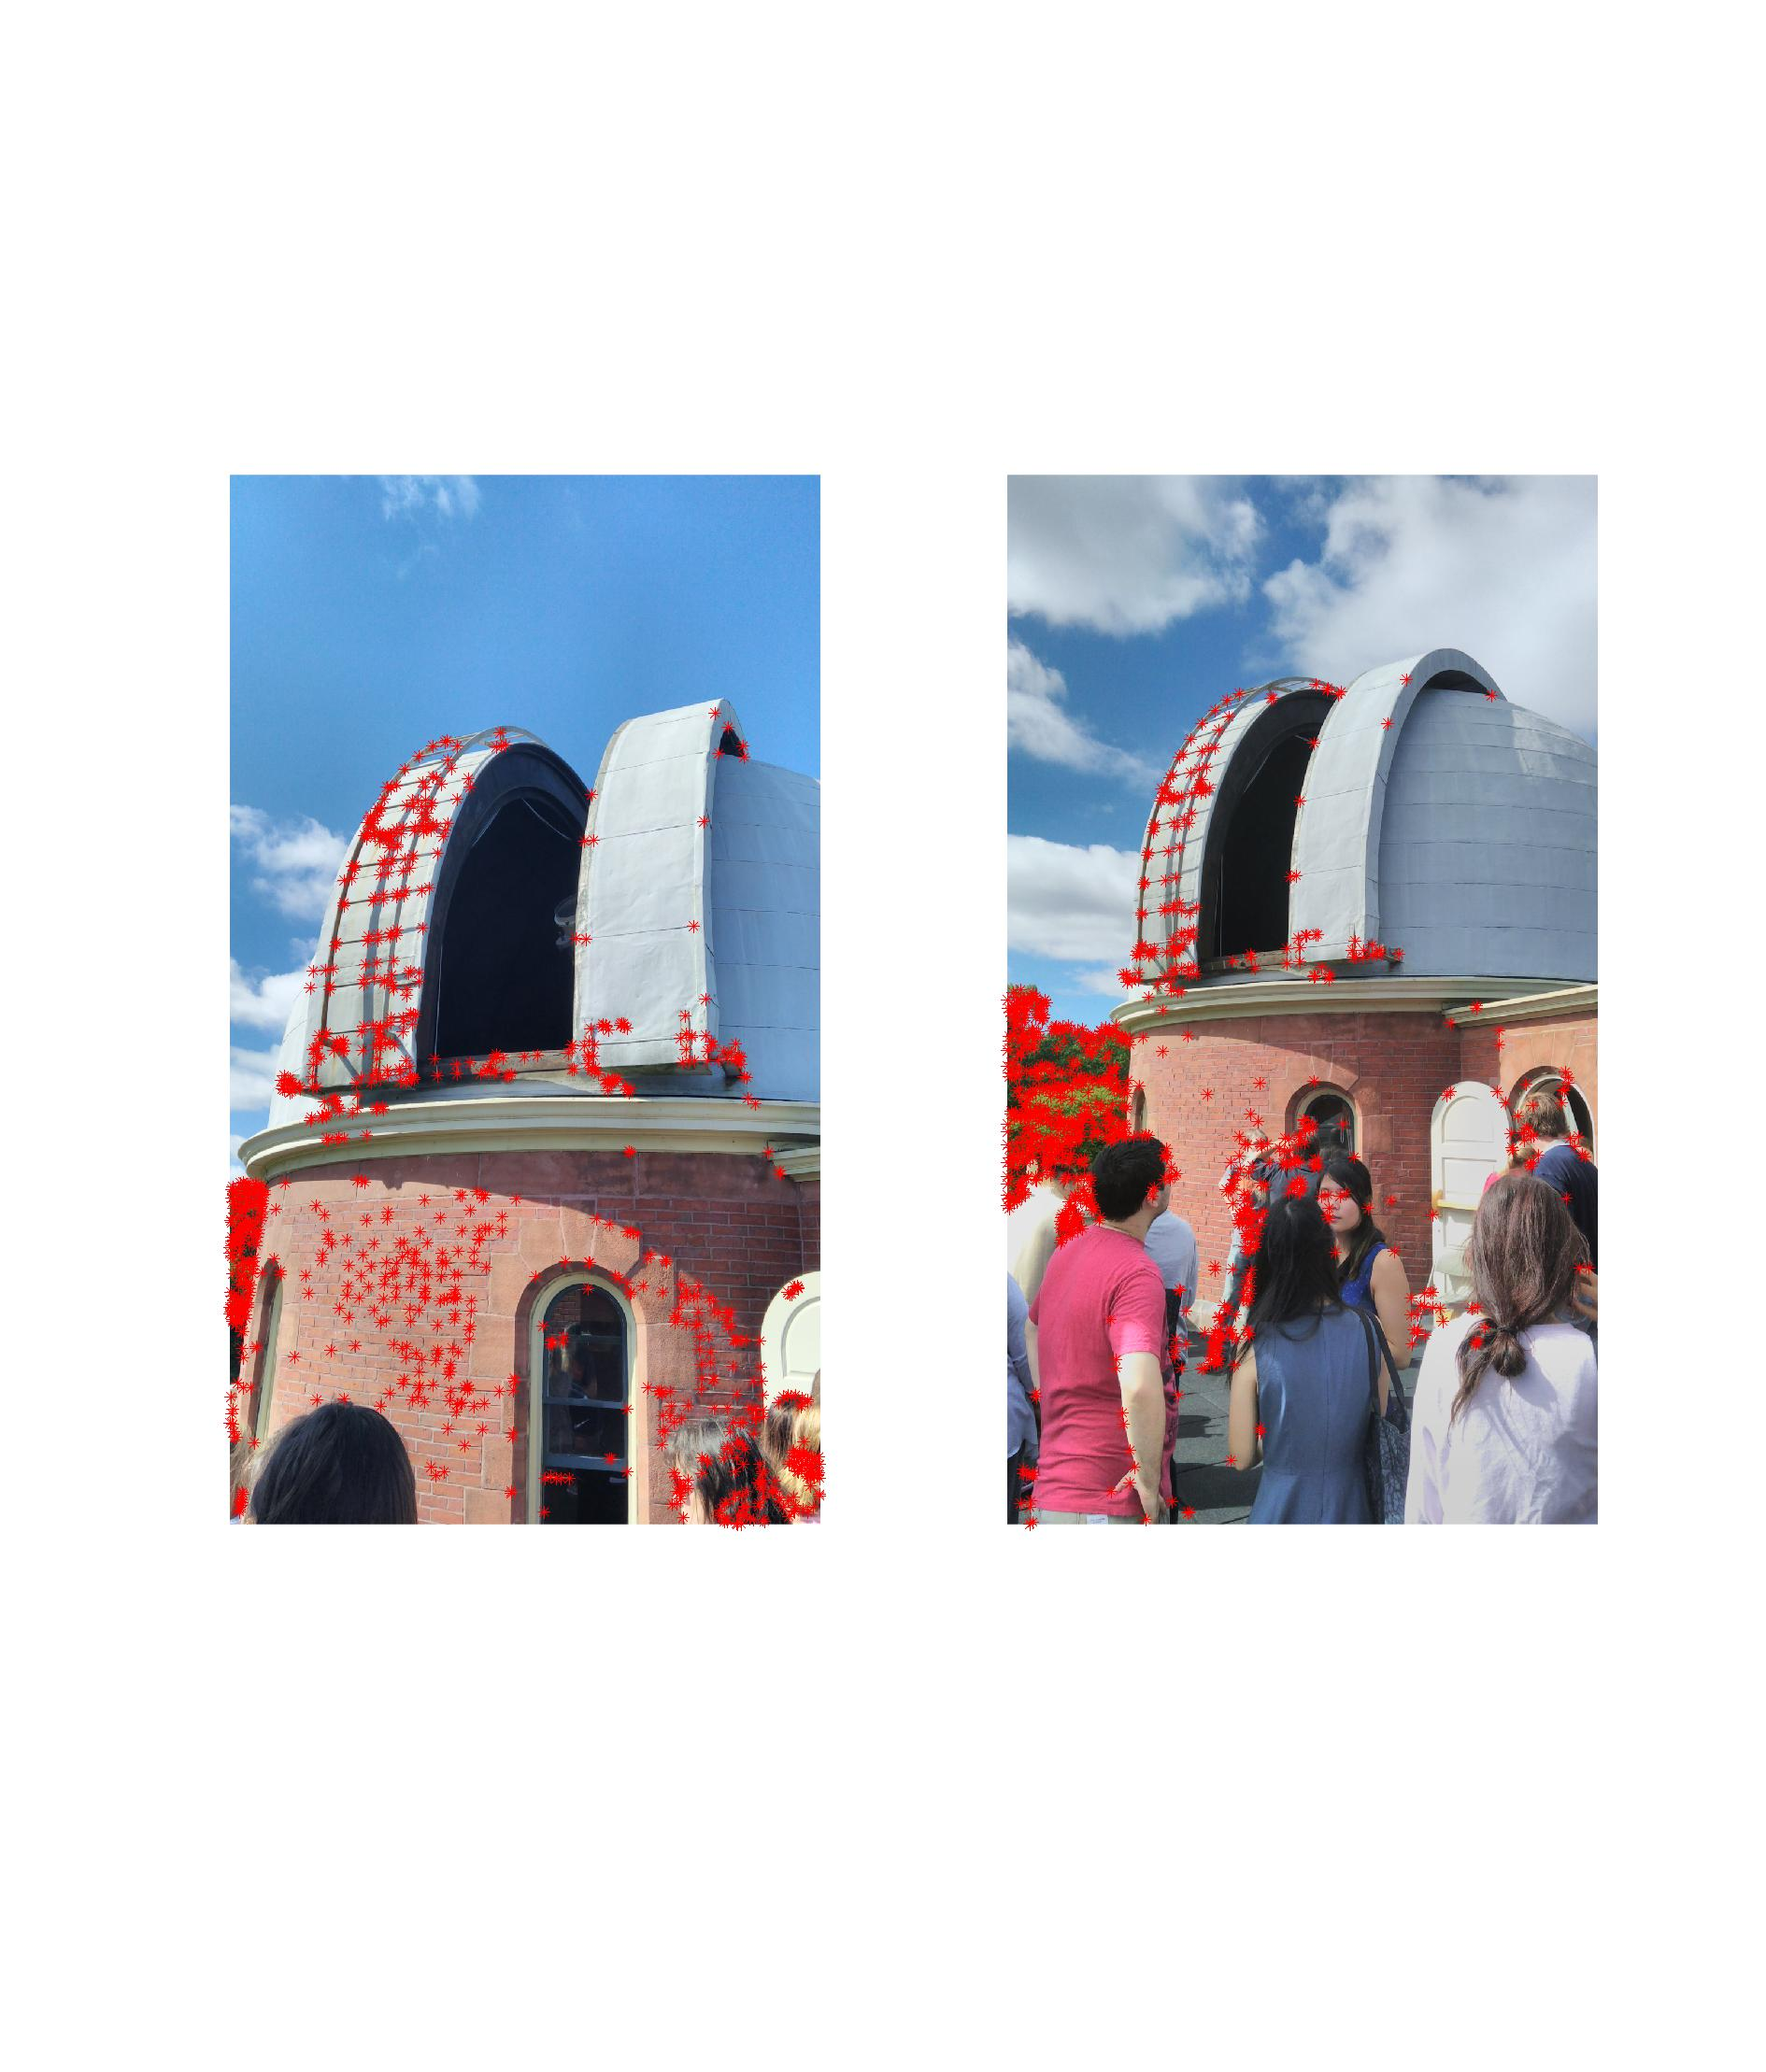
\includegraphics[width=5cm]{outputs/Observatory.jpg}
    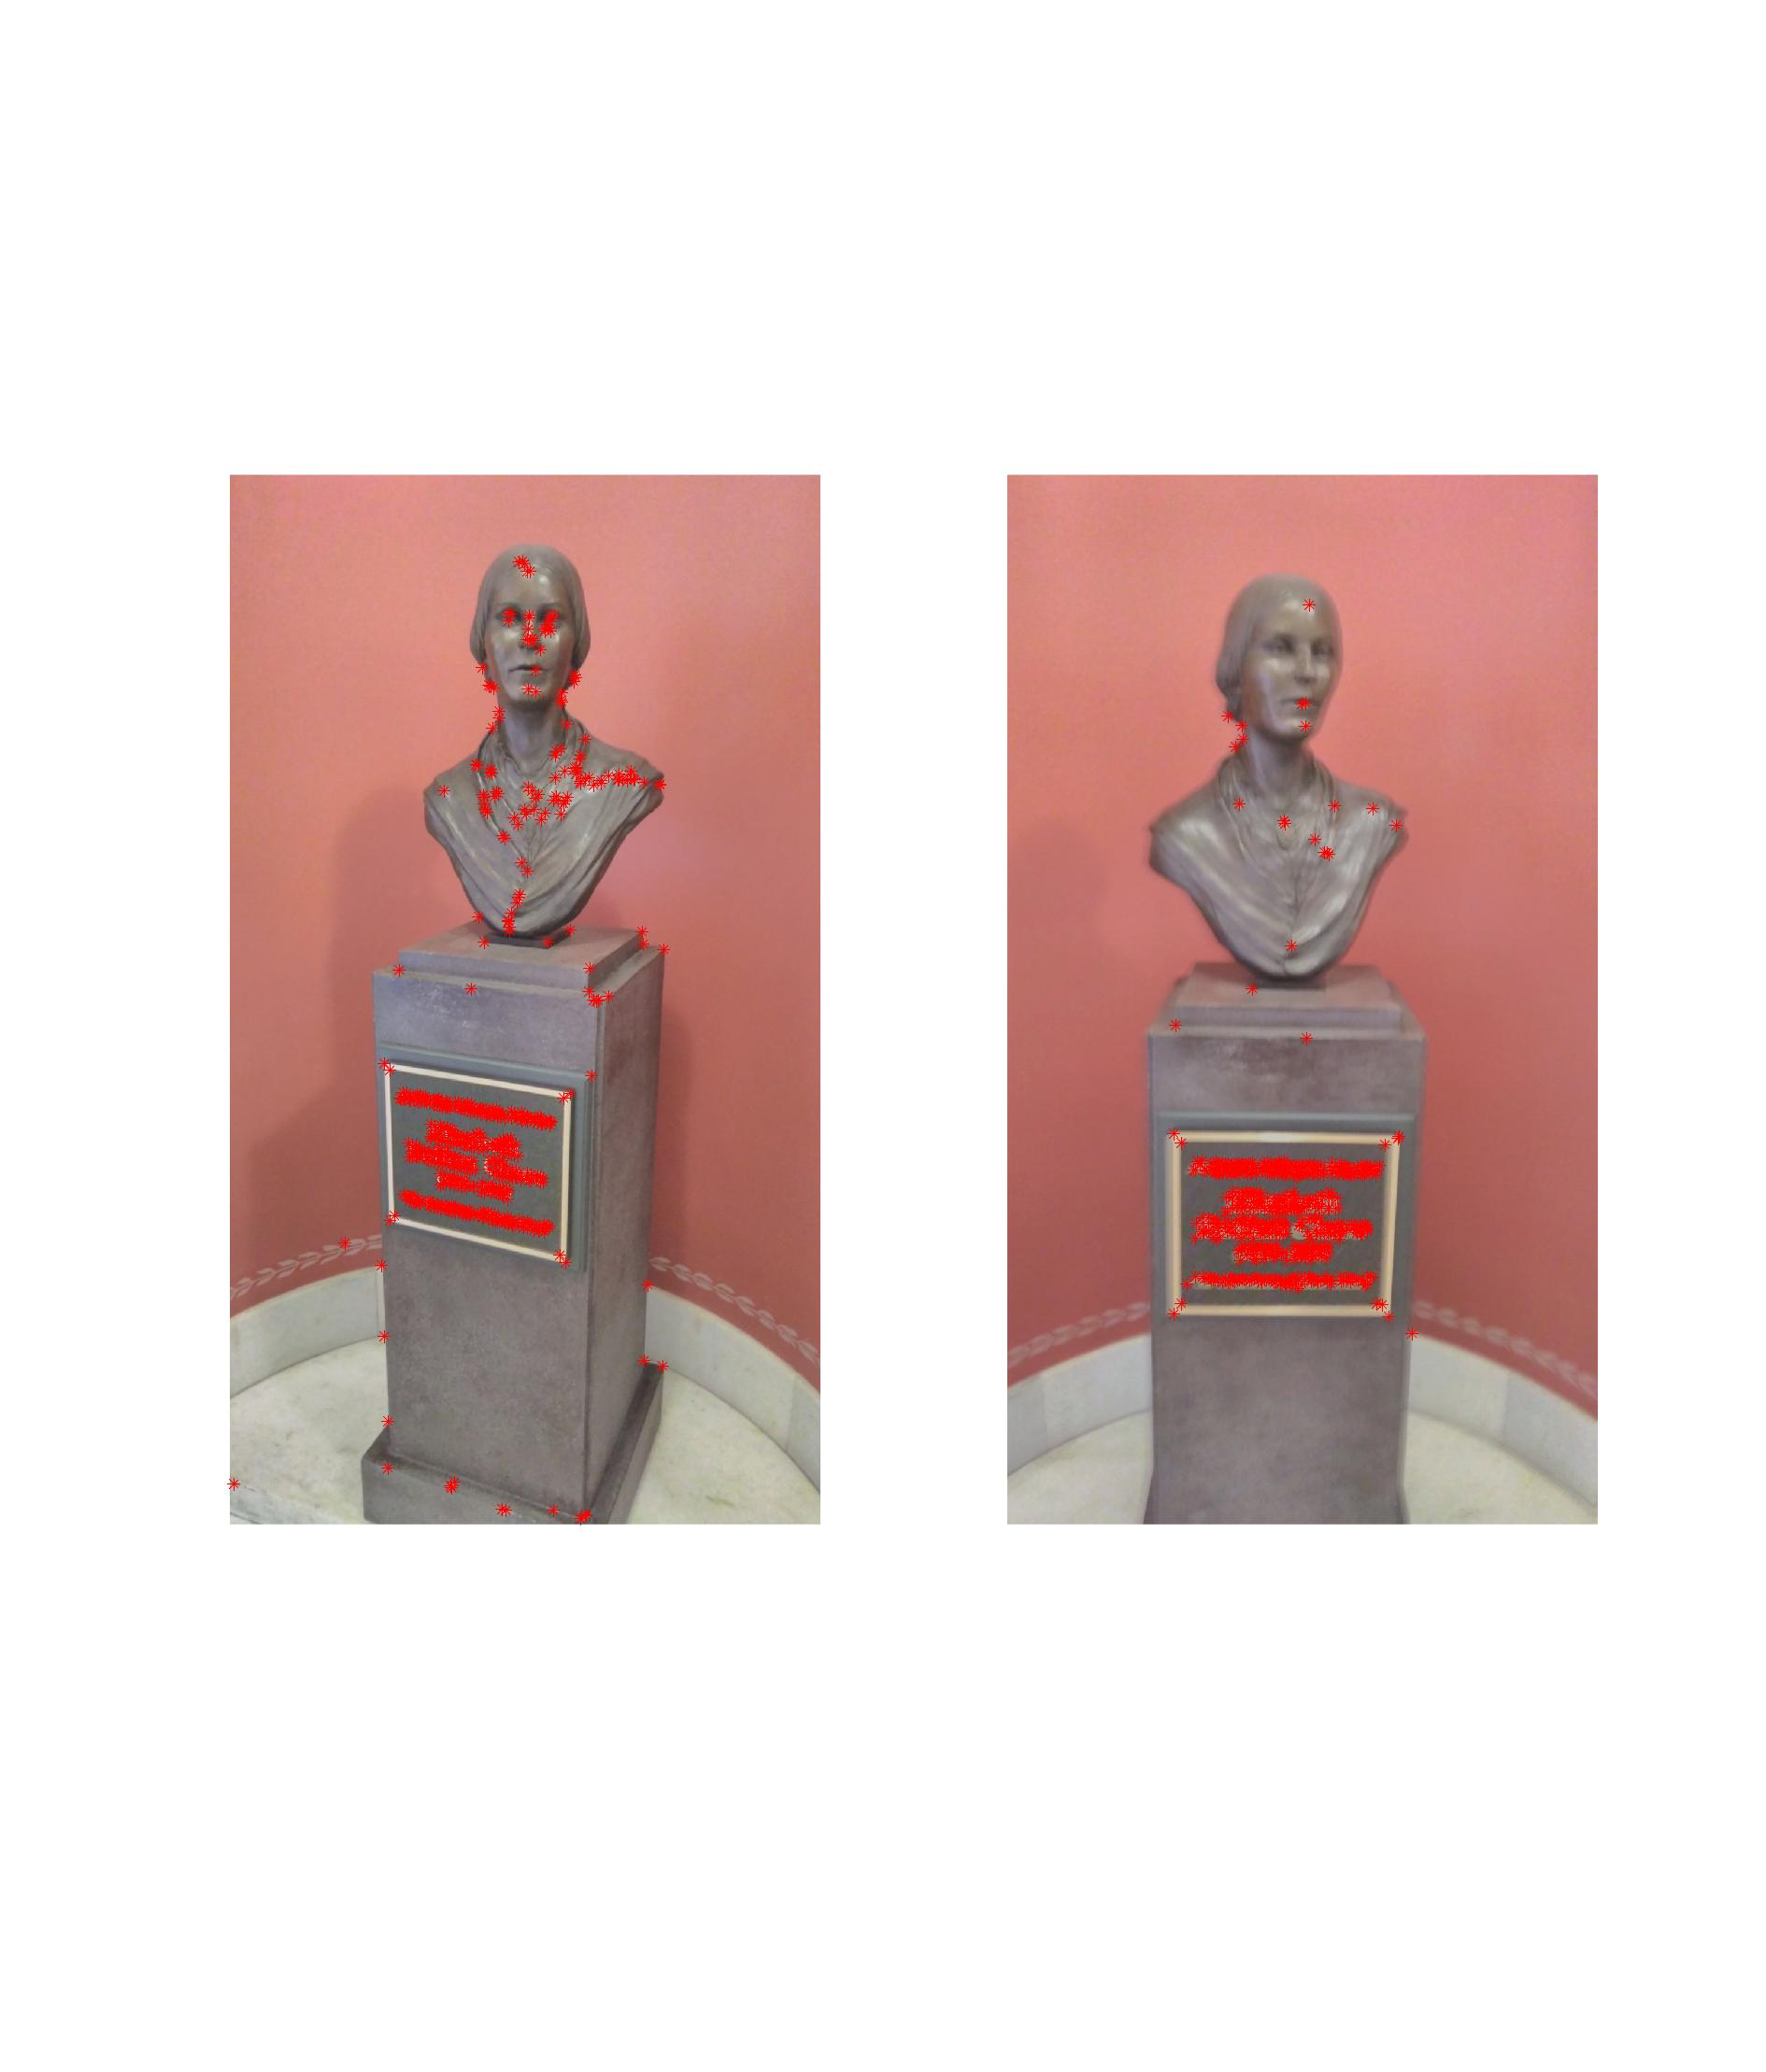
\includegraphics[width=5cm]{outputs/Chase.jpg}
    \caption{Corner detection outputs for image pairs}
    \label{fig:result1}
\end{figure}

%%%%%%%%%%%%%%%%%%%%%%%%%%%%%%%%%%%

% Please leave the pagebreak
\pagebreak
\paragraph{Q2:} In designing our feature point, what characteristics might we wish it to have? Describe the fundamental trade-off between feature point invariance and discriminative power. How should we design for this trade-off?

%%%%%%%%%%%%%%%%%%%%%%%%%%%%%%%%%%%
\paragraph{A2:}
We have seen from our lectures that some of the invariants we want for features involve invariance to transformation, scale, illuminance, chroma, and etc.. And to achieve invariance to these kinds of properties, we apply additional processing/normalizations to our images. From here, we can see that there is a trade-off between feature point invariance and discriminative power because processing and applying to much normalizations could eventually make two totally different features the similar. Therefore it is important to process features/images with just the right amount so that those kinds of side effects do not happen.

%%%%%%%%%%%%%%%%%%%%%%%%%%%%%%%%%%%

% Please leave the pagebreak
\pagebreak
\paragraph{Q3:} In the Harris corner detector, what do the eigenvalues of the `M' second moment matrix represent? Discuss both how they relate to image intensity and how we can interpret them geometrically.

%%%%%%%%%%%%%%%%%%%%%%%%%%%%%%%%%%%
\paragraph{A3:}
The second moment matrix provides the coefficients of the approximated E(u, v) function(auto-correlation function, as referred by the textbook). Therefore we can also say that they express the difference in intensity of two windows that are offsetted by (u, v).

If we were to consider a horizontal slice of the approximated \emph{E(u, v)}, the equation now expresses an ellipse. The eigenvalues of \emph{M} express the formation of that ellipse in that the length of the major and minor axis are expressed in terms of the two eigenvalues. This is significant because the shape of the ellipse determines whether the point is a corner or an edge or a regular area. We use this fact to calculate a value that helps us determine how confident we are about a point being a corner.

%%%%%%%%%%%%%%%%%%%%%%%%%%%%%%%%%%%


% Please leave the pagebreak
\pagebreak
\paragraph{Q4:} Explain the difference between the Euclidean distance and the cosine similarity metrics between descriptors. What might their geometric interpretations reveal about when each should be used? Given a distance metric, what is a good method for feature descriptor matching and why?

%%%%%%%%%%%%%%%%%%%%%%%%%%%%%%%%%%%
\paragraph{A4:}
Geometrically speaking, euclidean distance computes the distance between two points while cosine similarity computes the angle between two vectors. By the second law of cosine, we can observe that the euclidean distance takes into account the length of each vector as well as the angle between the two. On the other hand, cosine similarity only accounts for the angle difference between the two vectors. I believe that generally, euclidean distance can cover a more variety of situations since it takes more variables into account. So I think that euclidean distance has a slight edge in that regard. However, using cosine similarity on vectors that have consistent magnitudes(e.g. all vectors are unit vectors) can be better at times because it is easier to compute.
%%%%%%%%%%%%%%%%%%%%%%%%%%%%%%%%%%%


% If you really need extra space, uncomment here and use extra pages after the last question.
% Please refer here in your original answer. Thanks!
%\pagebreak
%\paragraph{AX.X Continued:} Your answer continued here.
\end{document}
